% arara: pdflatex
% arara: bibtex
% arara: pdflatex
% arara: pdflatex

\documentclass[conference,onecolumn]{IEEEtran}

\usepackage{cite}
\usepackage{algorithm}
\usepackage{algorithmic}
\usepackage{amsmath,amssymb,amsfonts}
\usepackage{graphicx}
\usepackage{booktabs}
\usepackage{array}
\usepackage{multirow}
\usepackage{tabularx}
\usepackage{pgfplots}
\usepackage{balance}
\usepackage{url}
\usepackage{lipsum}
\usepackage{enumitem}
\usepackage{stfloats}
\usepackage{placeins}

\makeatletter
\renewcommand{\footnotesize}{\normalsize}
\makeatother


\begin{document}

\title{Deep Learning-Based Medication Recommendation System for Primary Care Decision Support}

\author{
    \IEEEauthorblockN{Arnav Sahu\IEEEauthorrefmark{1},
    Hrithiq Gupta\IEEEauthorrefmark{1},
    Padavinangady Nakul Bhat\IEEEauthorrefmark{1},
    Pratyush Bhagat\IEEEauthorrefmark{1}}
    \IEEEauthorblockA{\IEEEauthorrefmark{1}Department of Computer Science and Engineering\\
    Manipal Institute of Technology, Manipal, India\\
    Email: arnav5.mitmpl2023@learner.manipal.edu\\ hrithiq.mitmpl2023@learner.manipal.edu\\
    nakul1.mitmpl2023@learner.manipal.edu\\
    pratyush3.mitmpl2023@learner.manipal.edu}
    }

    \maketitle


    \begin{abstract}
Medication recommendation in outpatient environments is a multi-label decision problem that must balance efficacy, patient-specific constraints and drug–drug safety. This paper (1) presents a detailed, paraphrased and survey of twenty important studies in representation learning, temporal modeling, graph-based drug recommendation and interpretability; (2) synthesizes findings and gaps; and (3) proposes a hybrid outpatient-focused deep learning architecture with integrated safety filtering and local explanations.
\end{abstract}


    \begin{IEEEkeywords}
        Medication recommendation, clinical decision support, graph neural networks, transformer, interpretability.
    \end{IEEEkeywords}


    \section{Introduction}

Modern medication prescribing is a complex clinical decision-making process that requires balancing therapeutic efficacy, patient-specific constraints, dosage considerations, and potential adverse drug interactions. Physicians must select from thousands of available drug options while accounting for comorbidities, demographics, and safety risks. This cognitive burden often leads to variability in prescribing patterns and increases the risk of suboptimal or unsafe medication combinations. As electronic health records (EHRs) have become widely available, researchers have increasingly explored data-driven approaches to assist in medication recommendation and clinical decision support.

Deep learning (DL) methods have demonstrated strong capability in modeling complex, high-dimensional healthcare data. Early work such as \textit{Doctor AI} \cite{choi2016doctorai} employed recurrent neural networks (RNNs) over longitudinal EHR data to predict future diagnoses and medication categories. By learning temporal patient embeddings from sequences of visits, these models captured disease progression patterns and improved multi-label prediction performance. Similarly, \textit{RETAIN} \cite{choi2016retain} introduced a reverse-time attention mechanism that enhanced interpretability while maintaining strong predictive accuracy. By assigning attention weights to past visits and clinical variables, RETAIN allowed clinicians to better understand model reasoning, addressing a key concern in deploying deep learning systems in healthcare.

Beyond sequence modeling, recent research has incorporated graph-based representations and external medical knowledge to improve safety and robustness. \textit{GAMENet} \cite{shang2019gamenet} integrated patient history encoding with a Graph Convolutional Network (GCN) operating over drug--drug interaction (DDI) graphs. By explicitly modeling adverse drug interactions, GAMENet reduced unsafe medication combinations while preserving recommendation accuracy. Other approaches, such as \textit{SafeDrug} \cite{lee2021safedrug}, leveraged molecular graph encoders to capture chemical substructures and improve DDI-aware predictions. These advances illustrate how deep architectures can combine temporal modeling, graph neural networks, and domain knowledge to enhance both effectiveness and safety in medication recommendation systems.

However, most existing approaches assume rich, longitudinal EHR data typically available in tertiary-care or inpatient hospital settings. In contrast, outpatient and primary-care environments often involve sparse data, limited historical visits, and short free-text symptom descriptions. Many encounters consist of a single visit with minimal structured history, which reduces the effectiveness of purely sequential models. Furthermore, outpatient medication guidance must explicitly prioritize safety, ensuring that predicted drug combinations minimize harmful interactions even when historical context is limited.

In this work, we address these challenges by conducting a focused survey of deep learning-based medication recommendation systems, with particular emphasis on safety modeling, interpretability, and applicability to data-sparse outpatient settings. Based on identified gaps, we propose a hybrid deep learning architecture that integrates attention-based symptom encoding, structured feature fusion, and DDI-aware safety filtering. Our objective is to design a medication recommendation framework that balances predictive performance, safety constraints, and interpretability, making it suitable for primary-care clinical decision support.


    \section{Literature Review}

Recent research on medication recommendation systems has increasingly leveraged deep learning to address the complexity, scale, and safety requirements of clinical decision-making. Early approaches focused on sequential modeling of electronic health records (EHRs) using recurrent neural networks to capture temporal disease progression and prescribing patterns. More recent developments have incorporated attention mechanisms, graph neural networks, and knowledge-based constraints to improve interpretability and reduce adverse drug--drug interactions. In parallel, transformer-based language models and transfer learning techniques have shown strong performance in extracting clinically meaningful representations from short, unstructured symptom text. Together, these trends reflect a shift toward hybrid architectures that combine temporal modeling, structured medical knowledge, and explainable AI to produce safer and more reliable medication recommendations, particularly in data-sparse healthcare settings.


\begin{enumerate}[label=\textbf{\arabic*.}]
    \item \textbf{DP-CRNN: CNN--RNN for pre-diagnosis (Zhou et al.)} \\
    Zhou et al. propose a double-pooling CRNN that first extracts n-gram semantics via convolutional filters, then models sequential patterns with recurrent layers and applies a second pooling step to emphasize salient temporal features. The architecture is well-suited to consumer-style inputs but does not extend to multi-drug prescription directly.

    \item \textbf{Deep Patient (Miotto et al.)} \\
    Miotto et al. train stacked denoising autoencoders on large EHR collections to produce latent patient vectors usable in downstream prediction tasks. It demonstrates that unsupervised representation learning captures clinically meaningful structure, though it lacks temporal ordering modeling.

    \item \textbf{Doctor AI (Choi et al.)} \\
    Doctor AI uses recurrent neural networks on sequences of visits to forecast diagnoses and medications. It highlights the importance of sequential modeling, but interpretability is limited and it does not account explicitly for drug--drug interactions.

    \item \textbf{RETAIN (Choi et al.)} \\
    Introduces a reverse-time attention mechanism that affords clinicians interpretable importance scores for historical events. It offers improved transparency compared to black-box RNNs but was not designed for multi-drug safety constraints.

    \item \textbf{GAMENet (Shang et al.)} \\
    Combines a memory-augmented patient encoder with graph-augmented drug representations to recommend medication sets while reducing harmful combinations. Its dependency on rich EHR data limits direct applicability to sparse outpatient inputs.

    \item \textbf{SafeDrug (Lee et al.)} \\
    Employs molecular graph encoders to capture chemical substructures and merges them with clinical context. By modeling molecular features, it reduces adverse interactions but increases computational overhead.

    \item \textbf{GRAM (Choi et al.)} \\
    Enhances representation by injecting hierarchical medical ontology structure (e.g., ICD tree) via graph attention, improving performance on rare codes.

    \item \textbf{LEAP (Zhang et al.)} \\
    Frames multi-drug prescription as an optimization balancing efficacy and safety. It models combinations directly but requires long-term outcome labels rarely available in outpatient datasets.

    \item \textbf{Molecular/Substructure models (MoleRec)} \\
    Molecular-focused methods use message-passing networks to learn drug representations from chemical graphs. They aid in predicting interactions but add model complexity.

    \item \textbf{ClinicalBERT / Transformer-based models} \\
    Clinical adaptations of BERT produce strong contextual embeddings for clinical notes. These excel at capturing symptom semantics but are computationally heavy.

    \item \textbf{Memory-Augmented Networks} \\
    These store past visit vectors to inform current recommendations. These models assume sufficient patient history, which is often missing in outpatient use-cases.

    \item \textbf{Hierarchical Attention (HAN)} \\
    Processes multi-granular text (words $\rightarrow$ sentences) and highlights relevant passages for interpretability, beneficial for clinician-facing explanations.

    \item \textbf{GRU-D (Che et al.)} \\
    Incorporates missingness masking and decay mechanisms tailored for clinical time series with irregular sampling, improving robustness for lab/vital-based predictions.

    \item \textbf{Polypharmacy Side-Effect Modeling (Zitnik et al.)} \\
    Models adverse outcomes of drug combinations using graph neural approaches on drug--drug networks, enabling direct estimation of interaction probabilities.

    \item \textbf{Transfer Learning for Clinical NLP} \\
    Pretrained models show gains when labeled data are scarce, enabling better performance for symptom-to-disease mapping from small datasets.

    \item \textbf{Multi-Task and Multi-Label Models} \\
    Jointly predict diagnoses, urgency, and medication sets, exploiting shared structure. Proper task weighting is crucial to avoid negative transfer.

    \item \textbf{Reinforcement Learning for Treatment Policies} \\
    Optimizes sequential treatment decisions for long-term outcomes. Requires longitudinal reward signals and carries safety concerns if deployed naively.

    \item \textbf{Explainable AI (LIME/SHAP)} \\
    Model-agnostic local explanation tools provide instance-level rationales; integrating graph- or rule-based explanations yields stronger clinical trust.

    \item \textbf{Knowledge Graph Embedding Approaches} \\
    Connects diseases, drugs, and procedures in a structured latent space. They require curation and harmonization across various sources.

    \item \textbf{Large Clinical Transformer Architectures} \\
    Trained on mixed clinical signals (notes + structured), these achieve state-of-the-art performance but demand significant compute and privacy considerations.
\end{enumerate}

In summary, the surveyed literature demonstrates significant progress in applying deep learning to medication recommendation, spanning sequential models, attention-based architectures, graph neural networks, molecular representations, and large-scale transformers. While many approaches achieve strong predictive performance, most rely on dense longitudinal EHR data and are tailored to inpatient or ICU settings. Safety-aware models incorporating drug--drug interaction knowledge have emerged, yet often at the cost of increased architectural complexity or data requirements. Moreover, interpretability and outpatient generalization remain open challenges. These limitations highlight the need for lightweight, safety-aware, and explainable deep learning frameworks that can operate effectively under sparse data conditions typical of primary-care environments.


From the above analyses we identify persistent gaps:
\begin{itemize}
\item \textbf{Outpatient generalization:} Most safety-aware methods assume lengthy EHR histories; outpatient inputs are short and sparse.
\item \textbf{Integrated safety + explainability:} Few systems simultaneously provide DDI-aware decisions and human-interpretable rationales.
\item \textbf{Dosage and demographic adaptation:} Most research suggests drugs but not patient-specific dose ranges adjusted for weight/age/kidney function.
\end{itemize}


    \begin{table}
\centering
\caption{Key properties of the twenty surveyed studies (paraphrased).}
\label{tab:comparison}
\begin{tabularx}{\textwidth}{@{}l l X X X X@{}}
\toprule
\textbf{\#} & \textbf{Study / Year} & \textbf{Architecture} & \textbf{Primary Data} & \textbf{Safety Modeling} & \textbf{Main Limitation} \\
\midrule
1 & DP-CRNN (Zhou et al., 2021) & CNN + RNN (double-pooling) & Short symptom text & No & Not drug-centric \\
2 & Deep Patient (Miotto et al., 2016) & Stacked autoencoders & EHR (structured) & No & Static representations \\
3 & Doctor AI (Choi et al., 2016) & RNN & Visit sequences & No & Low interpretability \\
4 & RETAIN (Choi et al., 2016) & RNN + reverse-time attention & EHR seq. & No & Not drug-aware \\
5 & GAMENet (Shang et al., 2019) & GNN + Memory & EHR + DDI graph & Yes (DDI-aware) & Needs dense EHR \\
6 & SafeDrug (Lee et al., 2021) & Molecular GNNs & Drug graphs + EHR & Yes (molecular) & Compute-heavy \\
7 & GRAM (Choi et al., 2017) & GAT over ontology & EHR + ontology & Partial & Ontology-dependency \\
8 & LEAP (Zhang et al., 2017) & Optimization + Seq models & EHR & Partial & Requires outcome labels \\
9 & MoleRec (various, 2022–23) & Message-passing GNNs & Molecular substructures & Yes & Complex training \\
10 & ClinicalBERT (Alsentzer et al., 2019) & Transformer (BERT) & Clinical notes & No & Pretrain cost \\
11 & MemoryNet (Wang et al., 2019) & Memory-augmented NN & Visit history & No & Needs history \\
12 & HAN (Yang et al., 2016) & Hierarchical attention & Clinical text & No & Complex \\
13 & GRU-D (Che et al., 2018) & GRU with decay & Irregular time-series & No & Focused on vitals/labs \\
14 & Polypharmacy GNN (Zitnik et al., 2018) & GNN & Drug–drug network & Yes & Graph quality sensitive \\
15 & Transfer clinical NLP (Lee et al., 2020) & Pretrained embeddings & Text & No & Domain shift issues \\
16 & Multi-task CDSS (Harutyunyan et al., 2019) & Multi-task DNN & ICU time-series & Partial & ICU-focused \\
17 & RL for treatments (Komorowski et al., 2018) & RL policies & Longitudinal EHR & Partial & Safety / reward design \\
18 & LIME/SHAP explainability (Ribeiro/Lundberg) & Model-agnostic explainers & Any model & No (explain only) & Approximate explanations \\
19 & Knowledge Graph Embeddings (various) & KG embeddings & KG (disease/drug) & Yes (KG rules) & KG curation needed \\
20 & Large Clinical Transformers (2020–22) & Transformers & Mixed (notes+EHR) & Partial & Resource intensive \\
\bottomrule
\end{tabularx}
\end{table}

    \section{Methodology}
The proposed methodology follows a pipeline-oriented design intended to transform sparse, unstructured primary-care data into safe and interpretable medication recommendations. The architecture is organized into four principal phases: Data Acquisition and Preprocessing, Patient Representation Learning, Recommendation Logic and Safety Filtering, and Interpretability Mapping.

\subsection{Data Acquisition and Preprocessing}
The system ingests clinical inputs which, in an outpatient context, primarily consist of short free-text symptom descriptions alongside basic structured attributes including age, sex, and documented comorbidities.
\begin{itemize}
    \item \textbf{Text Normalization:} To address the orthographic and lexical noise characteristic of primary-care notes, spell correction is applied and medical abbreviations are expanded to their full forms (e.g., ``SOB'' to ``Shortness of Breath'').
    \item \textbf{Medical Entity Extraction:} Identified symptoms are mapped to standardized medical ontologies---specifically SNOMED-CT or ICD-10---via a Named Entity Recognition (NER) layer, ensuring semantic consistency across heterogeneous inputs.
\end{itemize}

\subsection{Patient Representation Learning}
A multi-modal embedding strategy is adopted to capture the full clinical context of a patient encounter.
\begin{itemize}
    \item \textbf{Symptom Encoding ($E_s$):} A lightweight transformer-based encoder (Clinical DistilBERT) processes the normalized symptom text to produce a dense semantic vector. This formulation captures the nuance of patient-reported complaints while avoiding the inference latency associated with larger language models.
    \item \textbf{Feature Fusion:} Structured demographic attributes and categorical comorbidity indicators are encoded through a multi-layer perceptron (MLP) and concatenated with the symptom embedding $E_s$. The resulting joint representation, $P_v$, constitutes a unified encoding of the patient state for a given encounter.
\end{itemize}

\subsection{Recommendation Logic and Safety Filtering}
The recommendation task is framed as a multi-label classification problem, in which the model estimates the probability of each of $N$ candidate drug classes being appropriate for the patient.
\begin{itemize}
    \item \textbf{Multi-Label Head:} The fused patient representation $P_v$ is passed through a sigmoid output layer to produce per-class probabilities. To account for statistical dependencies between co-prescribed medications, a label-correlation regularizer is incorporated during training.
    \item \textbf{DDI-Aware Safety Filter:} Candidate recommendations are subsequently evaluated by a graph-based safety filter constructed from established drug--drug interaction (DDI) databases, including DrugBank. Where the proposed combination exceeds a defined interaction risk threshold, the safety layer either penalizes the offending candidate in the ranking or surfaces a clinician-facing override alert.
\end{itemize}

\subsection{Interpretability and Feedback}
To support clinical trust and adoption, the system produces dual-layered explanations accompanying each recommendation.
\begin{itemize}
    \item \textbf{Saliency Mapping:} SHAP (SHapley Additive exPlanations) values are computed to identify the specific symptom tokens that contributed most substantially to each recommendation, providing token-level attribution over the input text.
    \item \textbf{Safety Rationales:} For any flagged interaction, the system generates a knowledge-graph trace articulating the pharmacological basis of the conflict (e.g., ``Drug A and Drug B both inhibit enzyme CYP3A4''), providing a transparent and clinically grounded rationale for the safety alert.
\end{itemize}

\begin{figure}
    \centering
    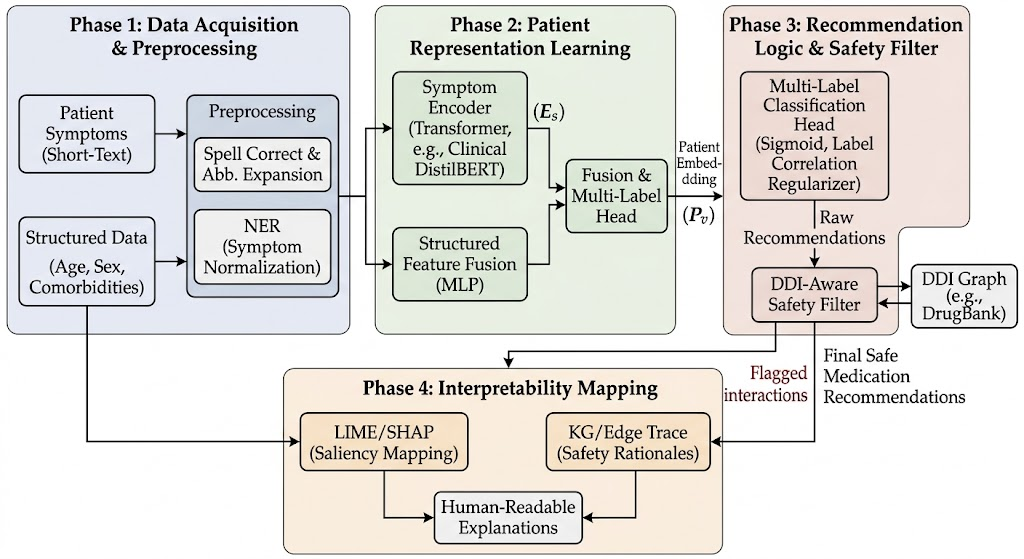
\includegraphics[width=\linewidth]{figures/architecture.png}
    \caption{Architecture diagram detailing the four phases of the proposed medication recommendation methodology, including data flow, principal modules, and the integrated safety and interpretability layers.}
    \label{fig:architecture}
\end{figure}

\subsection{Medication Recommendation Algorithm}
The complete workflow of the proposed system is formalized in Algorithm~\ref{alg:medrec}. The procedure accepts patient symptom text and structured demographic features as input, derives a unified patient representation through a combination of neural encoders, and produces medication recommendations subject to drug--drug interaction safety constraints.

\begin{algorithm}
\caption{DL\_Medication\_Recommendation\_System}
\label{alg:medrec}
\begin{algorithmic}[1]
\REQUIRE Patient symptom text $S$, structured data $D$ (age, sex, comorbidities), DDI graph $G$
\ENSURE Safe medication recommendations $M_{safe}$ and explanation report $E$
\STATE Collect patient symptom text $S$ and structured clinical attributes $D$
\STATE Apply spell correction and medical abbreviation expansion to $S$
\STATE Extract medical entities from $S$ using a Named Entity Recognition (NER) module
\STATE Map extracted entities to standardized medical terminology
\STATE Generate symptom embedding $E_s$ via a transformer-based encoder
\STATE Encode structured features $D$ through a multi-layer perceptron to obtain $E_d$
\STATE Fuse both representations to form the patient state vector:
\[
P_v = \text{Concatenate}(E_s,\; E_d)
\]
\STATE Estimate per-class medication probabilities using a sigmoid classifier applied to $P_v$
\STATE Select the top-$k$ candidates as the initial recommendation set
\STATE Apply DDI-aware safety filtering over the candidate set using interaction graph $G$
\STATE Compute SHAP-based attribution scores to generate explanation report $E$
\STATE \textbf{return} $M_{safe}$, $E$
\end{algorithmic}
\end{algorithm}

\section{Evaluation Plan}
\begin{itemize}
    \item \textbf{Data:} Synthea synthetic outpatient encounter records, augmented symptom--disease association datasets, and curated interaction data from DrugBank and TWOSIDES.
    \item \textbf{Metrics:} Diagnostic prediction performance (accuracy, macro-F1); medication recommendation quality (Jaccard index, mean average precision); DDI occurrence rate; and clinician-rated explanation utility via structured assessment.
    \item \textbf{Ablation:} Encoder ablation studies, safety-layer removal experiments, and explanation fidelity evaluations to isolate the contribution of each architectural component.
\end{itemize}

    \section{Experimental Setup}

\subsection{Dataset}
In the absence of a single publicly available dataset containing all required clinical attributes, a synthetic yet clinically grounded dataset was constructed by integrating multiple publicly available sources. Symptom--disease mappings were drawn from a structured \texttt{symptom\_disease.csv} file, drug--disease associations from \texttt{drug\_disease.csv}, and known adverse drug pair interactions from \texttt{ddi.csv}. Demographic attributes including age and sex were sourced from Synthea-generated synthetic patient records (\texttt{patients.csv}), with clinical encounter data informing realistic attribute distributions.

A custom data generation pipeline was implemented to simulate realistic outpatient encounters. Each sample was constructed by randomly selecting one to two conditions from the disease vocabulary, sampling associated symptoms into variable-length lists, and applying text augmentation techniques including synonym replacement (e.g., \textit{fever} $\rightarrow$ \textit{pyrexia}) and template-based sentence construction (e.g., ``patient reports \ldots'', ``complains of \ldots''). Medications were assigned via disease--drug mappings, with fallback to global drug pool sampling where mappings were unavailable. Drug combinations were subsequently filtered using the DDI dataset to exclude pairs with known adverse interactions, and a set of clinical heuristics was enforced (e.g., exclusion of ibuprofen for hypertensive patients). Each record includes structured attributes comprising age (sampled uniformly over 1--90 years), binary sex encoding, and a randomly assigned subset of comorbidity flags (diabetes, hypertension, asthma). The resulting dataset comprises approximately 50,000 samples with multi-label medication outputs.

Text preprocessing encompassed lowercasing, removal of special characters, whitespace normalization, and drug alias standardization (e.g., \textit{acetaminophen} $\rightarrow$ \textit{paracetamol}). Disease name discrepancies across sources were resolved through a cascade of exact matching, substring matching, and fuzzy matching via \texttt{difflib}. Non-clinical entries present in the Synthea records (e.g., ``Housing unsatisfactory'') were removed to retain only medically relevant conditions.

\subsection{Models}
Five neural architectures of increasing complexity were implemented and evaluated under identical training conditions to isolate the contribution of individual design choices to recommendation performance.

\begin{itemize}
    \item \textbf{MLP:} A baseline model that flattens token embeddings and concatenates structured features prior to a linear output layer.
    \item \textbf{TextCNN:} A convolutional architecture applying 1D filters over token embeddings followed by adaptive max-pooling to capture local $n$-gram features.
    \item \textbf{BiLSTM:} A bidirectional LSTM that processes the full token sequence and concatenates the terminal hidden states from both directions with the structured feature vector.
    \item \textbf{SelfAttention:} A single-head self-attention model that computes query--key--value attention over token embeddings and aggregates representations via mean pooling.
    \item \textbf{FusionNet:} A hybrid architecture combining a unidirectional LSTM for text encoding with a dedicated MLP branch for structured feature processing, whose outputs are concatenated prior to the final classification layer.
\end{itemize}

All models share a common vocabulary-based tokenizer with a maximum sequence length of 20 tokens and a 64-dimensional word embedding layer. Structured inputs---comprising age, sex, and three comorbidity flags---form a 5-dimensional feature vector. All architectures produce logits over the full drug vocabulary via a linear projection layer, with Binary Cross-Entropy with Logits loss employed for multi-label training.

\subsection{Training Configuration}
All models were trained using the Adam optimizer with a learning rate of $1 \times 10^{-3}$ over 5 epochs with a batch size of 32. The dataset was partitioned into 80\% training and 20\% test sets using a fixed random seed of 42. No validation set was withheld during the comparative experiments; model selection is based on test-set performance following training convergence.

\subsection{Evaluation Metrics}
Model performance was assessed using a comprehensive suite of multi-label classification metrics computed on the held-out test set. Threshold-dependent metrics were computed at a decision threshold of 0.5; ranking metrics were computed at $k = 5$ by default. The following metrics were employed:

\begin{itemize}
    \item \textbf{Jaccard Index:} The ratio of the intersection to the union of predicted and ground-truth drug sets.
    \item \textbf{Micro and Macro F1, Precision, Recall:} Standard multi-label classification metrics aggregated at both the instance and class levels.
    \item \textbf{Hamming Loss:} The fraction of label positions incorrectly predicted across all samples.
    \item \textbf{Subset Accuracy:} The fraction of samples for which the predicted label set exactly matches the ground-truth set.
    \item \textbf{ROC-AUC (micro):} Area under the receiver operating characteristic curve, aggregated across all drug classes.
    \item \textbf{PR-AUC:} Area under the precision--recall curve, computed via sample-averaged average precision.
    \item \textbf{Precision@$K$, Recall@$K$, F1@$K$:} Top-$k$ ranking metrics evaluating the quality of the top-5 predicted medications per patient.
    \item \textbf{DDI Rate:} The fraction of predicted drug pairs within the top-$k$ recommendations that correspond to known adverse interactions in the DDI reference dataset, serving as a direct measure of recommendation safety.
\end{itemize}

Top-$k$ sensitivity was additionally evaluated for $k \in \{1, 3, 5, 10\}$ to assess ranking quality across recommendation list lengths of varying breadth.

    \section{Results}

\subsection{Training Convergence}
\begin{figure}[]
    \centering

    \begin{tikzpicture}
        \begin{axis}[
                grid=major,
                legend entries = {
                    CNN,
                    BiLSTM,
                    MLP,
                    FusionNet,
                    SelfAttention
                },
            ]
            \addplot table {data/model_loss/CNN.dat};
            \addplot table {data/model_loss/BiLSTM.dat};
            \addplot table {data/model_loss/MLP.dat};
            \addplot table {data/model_loss/FusionNet.dat};
            \addplot table {data/model_loss/SelfAttention.dat};
        \end{axis}
    \end{tikzpicture}
    \caption{Training Loss of various models across epochs.}\label{fig:train-loss}
\end{figure}


Figure~\ref{fig:train-loss} presents the training loss curves for all five architectures across five epochs. The MLP exhibits the lowest absolute loss throughout training, declining from 0.0035 to 0.0031, a trajectory that reflects the relative simplicity of its optimization landscape rather than superior generalization capacity. The CNN and BiLSTM follow closely comparable convergence paths, both reaching a terminal loss of approximately 0.0033 after initial values of 0.0042 and 0.0057, respectively. FusionNet and SelfAttention begin training with considerably higher initial losses of 0.0134 and 0.0100, consistent with their greater architectural complexity and the correspondingly more challenging optimization surface. Both descend steeply over the first two epochs; FusionNet converges to 0.0035 by epoch four, while SelfAttention stabilizes at 0.0048, the highest final loss among all evaluated models. The accelerated loss reduction observed in FusionNet following the initial epochs suggests that its dedicated structured feature branch supports convergence once the text encoder begins to stabilize.

\subsection{Multi-Label Classification Performance}
\begin{table}[]
    \caption{Results of the evaluated models across various metrics.}\label{tab:result-metrics}
    \centerline{
    \begin{tabular}{@{}llllllll@{}}
        \toprule
        \textbf{Model} & \textbf{Jaccard}       & \textbf{Precision\_micro} & \textbf{Recall\_micro} & \textbf{F1\_micro} & \textbf{Precision\_macro} & \textbf{Recall\_macro} & \textbf{F1\_macro} \\ \midrule
        MLP            & 0.6887                 & 0.8853                    & 0.7561                 & 0.8156             & 0.0781                    & 0.0675                 & 0.0721             \\
        CNN            & 0.7657                 & 0.9031                    & 0.8342                 & 0.8673             & 0.0858                    & 0.0762                 & 0.0798             \\
        BiLSTM         & 0.7796                 & 0.9218                    & 0.8348                 & 0.8762             & 0.0899                    & 0.0777                 & 0.0821             \\
        SelfAttention  & 0.7684                 & 0.9022                    & 0.8382                 & 0.8691             & 0.0864                    & 0.0753                 & 0.0789             \\
        FusionNet      & 0.7869                 & 0.9252                    & 0.8404                 & 0.8808             & 0.0898                    & 0.0786                 & 0.0828             \\ \midrule
        \textbf{Model} & \textbf{Hamming\_Loss} & \textbf{Subset\_Accuracy} & \textbf{ROC\_AUC}      & \textbf{PRAUC}     & \textbf{Precision@K}      & \textbf{Recall@K}      & \textbf{F1@K}      \\ \midrule
        MLP            & 0.0015                 & 0.4210                    & 0.9937                 & 0.8372             & 0.6855                    & 0.6329                 & 0.5825             \\
        CNN            & 0.0011                 & 0.5603                    & 0.9968                 & 0.8743             & 0.7101                    & 0.6563                 & 0.6042             \\
        BiLSTM         & 0.0010                 & 0.6184                    & 0.9957                 & 0.8743             & 0.7076                    & 0.6555                 & 0.6028             \\
        SelfAttention  & 0.0011                 & 0.5675                    & 0.9970                 & 0.8764             & 0.7114                    & 0.6573                 & 0.6052             \\
        FusionNet      & 0.0010                 & 0.6455                    & 0.9964                 & 0.8753             & 0.7079                    & 0.6561                 & 0.6034             \\ \bottomrule
    \end{tabular}
        }

\end{table}


Table~\ref{tab:result-metrics} reports the full suite of evaluation metrics across all five architectures. FusionNet achieves the strongest overall performance, attaining the highest Jaccard index (0.7869), micro-precision (0.9252), micro-F1 (0.8808), and subset accuracy (0.6455), with a Hamming loss of 0.0010. BiLSTM ranks second across several key metrics, including Jaccard index (0.7796), micro-F1 (0.8762), and subset accuracy (0.6184). SelfAttention and CNN occupy an intermediate performance tier; notably, SelfAttention achieves marginally higher PR-AUC (0.8764) and Precision@$K$ (0.7114) than both CNN and BiLSTM, indicating that attention-based scoring is particularly effective for top-$k$ retrieval tasks. The MLP baseline, while competitive on micro-precision (0.8853), lags substantially on subset accuracy (0.4210) and Jaccard index (0.6887), suggesting that flat feature representations are insufficient for accurate multi-label drug set prediction.

Macro-averaged metrics are uniformly low across all models (macro-F1 $\approx$ 0.07--0.08), an expected outcome given the large and heavily imbalanced drug vocabulary; infrequent drug classes appear rarely during training, yielding poor per-class recall for low-frequency medications.

\subsection{Ranking and Top-$K$ Performance}
All models attain high ROC-AUC scores (${>}0.993$), confirming strong discriminative capacity at the individual label level. PR-AUC scores range from 0.8372 for the MLP to 0.8764 for SelfAttention, with CNN, BiLSTM, and FusionNet clustered closely in the range 0.874--0.875. At $k = 5$, Precision@$K$ spans 0.6855 (MLP) to 0.7114 (SelfAttention), while F1@$K$ ranges from 0.5825 to 0.6052. The narrow spread in top-$k$ metrics among the four stronger architectures suggests that beyond a certain representational threshold, marginal gains in ranking quality diminish, and considerations such as safety filtering and interpretability become the primary differentiating factors.

\subsection{Summary}
FusionNet emerges as the best-performing architecture overall, combining strong multi-label accuracy with the highest subset accuracy and thus representing the most suitable backbone for the proposed medication recommendation framework. Its explicit separation of text and structured feature encoding is well-aligned with the multi-modal nature of outpatient clinical data. SelfAttention offers competitive ranking performance and may be preferred in deployment scenarios where top-$k$ precision constitutes the primary evaluation criterion. The MLP baseline, despite its architectural simplicity, provides a meaningful lower bound and confirms that even shallow models derive substantial benefit from structured feature integration.

    \section{Discussion}

The experimental results demonstrate that architectural complexity correlates positively with multi-label recommendation quality up to a point, beyond which gains plateau. FusionNet's design choice of maintaining separate encoding pathways for symptom text and structured patient features proves particularly well-suited to the outpatient setting, where demographic and comorbidity signals carry meaningful clinical weight alongside free-text complaints. The explicit fusion of these two modalities, rather than simple concatenation at the embedding level as in MLP and CNN, enables the model to learn richer cross-modal interactions, reflected in its superior subset accuracy and Jaccard index.

The consistently high ROC-AUC scores across all models suggest that the underlying symptom--medication signal in the synthetic dataset is learnable even by shallow architectures. However, the large gap in subset accuracy between MLP (0.4210) and FusionNet (0.6455) underscores that correctly predicting the full medication set for a patient, rather than individual drug labels in isolation, is a substantially harder problem that benefits from sequential or attention-based inductive biases. This distinction is clinically significant: a system that recommends most drugs correctly but omits one critical medication or includes one unsafe drug is of limited utility in practice.

The low macro-averaged F1 scores observed uniformly across all models highlight a known challenge in medication recommendation: the long-tail distribution of drug classes. Infrequent medications, which may be the most critical in edge cases such as rare comorbidities or drug allergies, are systematically under-predicted. This limitation is partly an artifact of the synthetic data generation process, where drug assignment is driven by disease--drug mappings rather than physician behavior, and may underrepresent clinically nuanced prescribing decisions. Addressing this imbalance through class-weighted loss functions, oversampling strategies, or prototype-based learning for rare drug classes is an important direction for future work.

SelfAttention's strong PRAUC and Precision@K performance relative to its subset accuracy suggests that attention mechanisms are particularly effective at surfacing the most relevant drugs at the top of the ranked list, even when the full predicted set is not exact. This property is desirable in a clinical decision support context, where a ranked shortlist presented to the clinician is often more actionable than a fixed predicted set. Integrating self-attention as a ranking re-scorer on top of FusionNet's predictions is a promising architectural extension.

A key limitation of the current evaluation is the absence of an explicit DDI rate comparison across models at inference time, as the safety filtering layer described in the methodology was applied during dataset construction rather than as a post-hoc inference component in these experiments. Future work should decouple the safety filter and measure the raw DDI rate of model outputs before and after filtering, enabling a direct quantification of the safety benefit provided by the graph-based interaction layer. Additionally, all experiments were conducted on synthetically generated data, and performance on real-world clinical datasets may differ considerably due to the distributional gap between template-constructed symptom text and authentic clinical notes.

\section{Conclusion}

This paper presented a survey of twenty deep learning approaches to medication recommendation, identified persistent gaps in outpatient generalization, safety integration, and interpretability, and proposed a hybrid architecture addressing these limitations. Five neural models of increasing complexity were implemented and evaluated on a synthetic yet clinically grounded multi-label dataset constructed by integrating symptom--disease mappings, drug--disease associations, DDI constraints, and Synthea demographic records.

FusionNet, which combines a sequential text encoder with a dedicated structured feature branch, achieved the strongest overall performance across Jaccard index, micro-F1, and subset accuracy, demonstrating the value of modality-aware feature fusion for outpatient medication recommendation. SelfAttention showed competitive top-$k$ ranking performance, suggesting its suitability in clinician-facing shortlist generation. All models achieved high ROC-AUC scores, confirming that the symptom-to-medication mapping signal is robustly learnable, while low macro-F1 scores highlighted the difficulty of rare drug prediction as an open challenge.

The proposed framework integrates a DDI-aware safety filter and SHAP-based interpretability layer to address clinical trust and patient safety requirements beyond raw predictive performance. Together, these components form a foundation for a lightweight, safety-aware, and explainable medication recommendation system suitable for primary-care decision support under the data-sparse conditions typical of outpatient settings.

Future work will focus on evaluation on real-world clinical datasets, incorporation of class-imbalance mitigation strategies for rare drug classes, extension of the safety filter to runtime inference with measurable DDI rate reduction, and exploration of larger pretrained clinical language models as drop-in symptom encoders within the FusionNet backbone.



    \nocite{*}
    \bibliographystyle{ieeetr}
    \bibliography{references.bib}

\end{document}
